En este capítulo se describen los principales conocimientos sobre vídeos relacionados con el objetivo principal de este trabajo. En primer lugar se detalla el proceso de generación de un vídeo y su composición basada en imágenes para luego hablar de los métodos más habituales de compresión para el almacenamiento del mismo. Una vez explicado este proceso se comentará cómo interviene el tipo de sensor en la extracción del ruido del dispositivo.

\section{Proceso de generación de un vídeo digital}
El proceso de generación de un vídeo digital está basado en transformar se\~nales analógicas (funciones con dominio continuo y que toman valores en un conjunto continuo) en se\~nales digitales, capaces de ser procesadas por un ordenador. Para convertir una se\~nal analógica en una se\~nal digital (conversión A/D) se utilizan dos técnicas: muestreo y cuantificación.
\subsection{Muestreo}
El proceso de muestreo o \textit{sampling} consiste en transformar una se\~nal con dominio continuo en otra de dominio discreto, de forma que se retenga el máximo posible de la información original de la se\~nal analógica. Gráficamente se puede ver un ejemplo de muestreo en \ref{fig_muestreo}.

\begin{figure}[ht!]
\begin{center}
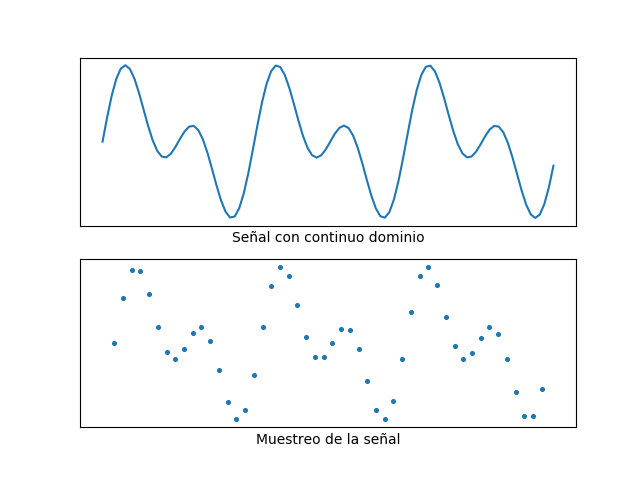
\includegraphics{figuras/muestreo.png}
\end{center}
\caption{Muestro de una se\~nal de dominio continuo}
\label{fig_muestreo}
\end{figure}

La técnica del muestreo ha sido ampliamente estudiada pues es usada en una gran variedad de campos y existen métodos y fórmulas matemáticas para determinar cotas inferiores que no elimenen información del original, sin embargo en este contexto hay cotas menos exigentes debido a la capacidad que tiene el cerebro para procesar visualmente un objeto. 
En el contexto de este trabajo hay dos tipos diferentes que se deben realizar: uno asociado a las variables espaciales y otro asociado al tiempo. Ambos casos se basan en tener muestras muy cercanas de forma que la composición parezca continua y no discreta.
El muestro de la variable temporal está relacionado con el número de imágenes por segundo que es capaz de procesar el ojo humano, estando entre 25 y 30 lo que el ojo ya percibe como continuo.
Al discretizar la sen\~al analógica obtenemos un conjunto finito que podemos numerar y expresar en forma de una matriz de dos dimensiones, siendo cada una de las celdas un pixel (del inglés \textit{picture element}). Para el número de filas y columnas elegido por el muestro se toma un múltiplo de dos, puesto que tiene por una parte la ventaja de favorecer el direccionamiento de las muestras y por otra de ser más eficientes para ciertos algoritmos como puede ser la transformada de Fourier.
En el muestro también interviene la frecuencia de la se\~nal original: una con baja frecuencia puede ser bien representada con una tasa de muestreo determinada, pero la misma puede ser no válida para una frecuencia alta, produciéndose el efecto que conocemos como solapamiento o \textit{aliasing}. El teorema de Nyquist establece que utilizando una tasa de muestro mayor al doble de la frecuencia original, se evita el \textit{aliasing} y se puede recuperar la se\~nal original a partir de la transformada. En \ref{fig_nyquist} se puede observar como cuando la frecuencia de muestreo es suficientemente grande comparado con la frecuencia original (figura de arriba) se puede reconstruir la onda original, mientras que en la figura de abajo se observa que cuando no se cumple el Teorema de Nyquist se produce una pérdida de información que impide reconstruir la se\~nal original\cite{b3:2012}.

\begin{figure}[ht!]
\begin{center}
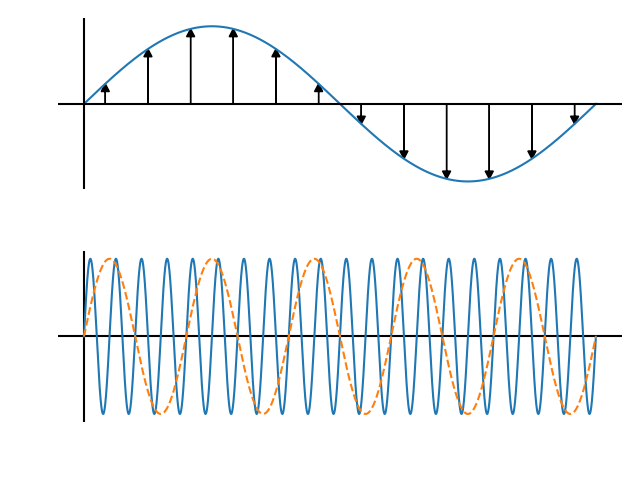
\includegraphics{figuras/nyquist.png}
\end{center}
\caption{Frecuencia en el muestreo}
\label{fig_nyquist}
\end{figure}

\subsection{Cuantificación}
La cuantificación consiste en transformar el rango continuo de la se\~nal analógica en un rango discreto. La intensidad que es una se\~nal continua es transformada a un conjunto finito que son los valores que pueden tomar los pixels. De esta forma, mientras que con el muestro reducimos una variable espacial continua en una matrix, la cuantificación permite que la intensidad que capta la lente del dispostivo se pueda representar por un conjunto discreto de valores. 
De la misma forma que en el muestreo, se suele utilizar un conjunto de cardinalidad potencia de dos. Para imágenes en color lo usual es trabajar con tres componentes cada uno de ocho bits, mientras que en las imágenes en blanco y negro se trabaja con un componente de ocho bits. 
Cabe destacar que este proceso no es reversible y está asociado a funciones no lineares, al contrario que el muestro, en el que partiendo de premisas no muy exigentes se puede reconstruir la se\~nal analógica. \\

El proceso de cuantificación en vídeo se basa en aplicar frame a frame el método que se aplica en JPEG. En primer lugar se divide la imagen o frame en bloques disjuntos de $8$x$8$ pixels, para cada uno de estos bloques $B$ se calcula la transformada del coseno discreta (DCT) siguiendo\cite{fridrich:2003}:

\begin{equation}
D_{ij} = \sum_{k,l=0}^{7}a_{kl}(i,j)B_{kl} \nonumber
\end{equation}

donde
\begin{equation} \label{eq:dct}
a_{kl}(i,j) = \frac{1}{4}w(k)w(l)\cos\frac{\pi}{16}k(2i+1)\cos\frac{\pi}{16}k(2j+1) 
\end{equation}

y

\begin{equation}
w(k) = 
\begin{cases}
\frac{\displaystyle 1}{\displaystyle\sqrt{2}} & \text{si $k=0$}\\
1 & \text{en caso contrario} \nonumber
\end{cases}
\end{equation}

Aplicando DCT se transforma la fuente original en el dominio de las frecuencias. Los coeficientes $a_{kl}$ de la ecuación \ref{eq:dct}, multiplicadores de los valores del bloque de la imagen, cumplen que a medida que nos distanciamos de la primera fila se incrementa la varianza, como podemos ver en \ref{fig_dct}. Además, a medida que nos distanciamos de la primera columna también crece la varianza. Por otra parte, los coeficientes DCT que se corresponden con frecuencias bajas son grandes en magnitud.

\begin{figure}[ht!]
\begin{center}
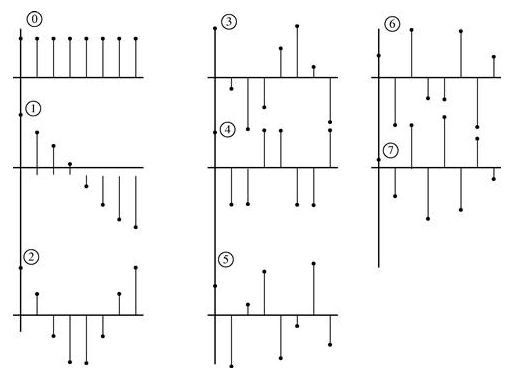
\includegraphics[width=10cm,height=10cm,keepaspectratio]{figuras/dct.png}
\end{center}
\caption{Varianza según la fila del bloque en la transformada DCT, \cite{b4:2012}}
\label{fig_dct}
\end{figure}


La matriz $D$ con los coeficientes DCT es discretizada posteriormente utilizando una matriz de cuantificación $Q$, producto de una tabla de valores y cuantificación y una escala de cuantificicación, fija en el caso de una tasa de bits variable (VBR) y variable en el caso de una tasa de bits constante (CBR). 
\begin{equation}
D_{ij} = round\left(\frac{D_{ij}}{Q_{ij}}\right),  i,j\in\{0, \dots, 7\} \nonumber
\end{equation}

En la matriz de cuantificación, cada elemento define el umbral bajo el cual un detalle en la imagen debe ser capturado como tal o descartado. De esta forma, a medida que nos alejamos del origen, ya sea horizontal o verticalmente, se exige un mayor coeficiente DCT para que el detalle sea relevante, puesto que se corresponden con valores de mayor frecuencia. Hay una gran variedad de matrices de cuantificación, calculadas normalmente en base a experimentos psico-visuales para determinar los umbrales DCT. Una matriz de cuantificación ampliamente utilizada es la siguiente\cite{b3:2012}:
$$
\begin{bmatrix}
8 & 16 & 19 & 22 & 26 & 27 & 29 & 34 \\
16 & 16 & 22 & 24 & 27 & 29 & 34 & 37 \\
19 & 22 & 26 & 27 & 29 & 34 & 34 & 38 \\
22 & 22 & 26 & 27 & 29 & 34 & 37 & 40 \\
22 & 26 & 27 & 29 & 32 & 35 & 40 & 48 \\
26 & 27 & 29 & 32 & 35 & 40 & 48 & 58 \\
26 & 27 & 29 & 34 & 38 & 46 & 56 & 69 \\
27 & 29 & 35 & 38 & 46 & 56 & 69 & 83 \\
\end{bmatrix}
$$

\section{Almacenamiento de vídeos digitales}
Del proceso descrito en la sección anterior, es fácil deducir que la cantidad de datos en se\~nales visuales es grande. Una imagen en blanco y negro de dimensiones $M$x$N$ con $B$ bits para el nivel de resolución del gris supone un tama\~no de $NMB$ bits. Esto supone que una sola imagen de color de $512$ x $512$ x $8$ ocupa cerca de 1MB. Esto implica que un vídeo con estas características y una tasa de muestro de 30 frames por segundo (el mínimo para que el ojo humano lo detecte como continuo) requiere 23.6MB por segundo\cite{b2:2005}.\\

Esta gran cantidad de datos que sería necesaria para almacenar un vídeo no solamente supone un problema en cuanto a requisitos de memoria, si no también para el procesamiento y trasmisión de los mismos. Como consecuencia, es necesario reducir la cantidad de datos mediante algoritmos de compresión, que en el caso de vídeos están definidos por el comité MPEG (del inglés \textit{Moving Pictures Expert Group}) de forma estándar e internacional.
Como ya se ha comentado anteriormente, se puede ver un vídeo como una sucesión de imágenes o \textit{frames}. Además de aprovechar la compresión de imágenes, en el caso del vídeo se tiene una redundancia temporal ya que el siguiente frame tiene mucho en común con el actual y los anteriores, factor que se aprovechará para reducir el tama\~no. \\

Los algoritmos de codificación más utilizados han sido definidos por un grupo de expertos conocido como MPEG (del inglés \textit{Motion Picture Expert Group}) y se basan, al igual que la mayoría de algoritmos de compresión de vídeo en el concepto llamado grupo de imágenes o GOP (del inglés \textit{Group Of Pictures}). Un GOP de tama\~no $N$ está compuesto de $N$ imágenes que pueden ser de tipo:
\begin{itemize}
\item Los \textbf{I-frames} o \textit{intra-coded frames} se codifican de forma independiente, sin referencias a otros frames. Esto permite acceso aleatorio a los datos del vídeo, puesto que pueden ser decodificados sin necesitar de otros frames. Además de esto, tienen la ventaja de evitar la propagación de errores que se acarrea en la compresión de frames consecutivos al contener la mayor información de la escena por si solos, a costa de ocupar más que los otros tipos de frames. En cada GOP debe constar al menos un I-frame.
\item Los \textbf{P-frames} son frames pronosticados, comprimidos basados en la diferencia que existe respecto de un I-frame o P-frame anterior.
\item Los \textbf{B-frames} son frames bidireccionales que usan los datos de imágenes previas y posteriores de I-frames o P-frames.
\item Los \textbf{D-frames} son frames de baja resolución que raramente se utilizan y que se obtienen decodificando el coeficiente $dc$ de la transformada de coseno discreta (DCT) de los coeficientes de cada macrobloque.
\end{itemize} 

En cuanto a la compresión:
\begin{itemize}
\item Los I-frames se comprimen mediante el uso de la transformada del coseno discreta y la cuantificación, de la misma forma que en el caso de imágenes, puesto estos frames deben contener toda la información relevante de manera aislada. Se comprime por separado la luminosidad y la crominancia.
\item En el caso de los P-frames la compresión depende de la similitud entre el frame en cuestión y los del grupo en que se encuentra. Si no se encuentra un frame adecuado, este deberá comprimirse del mismo modo que si se tratase de un I-frame. En caso de encontrarse un buen candidato, se computa el residuo entre ambos y se cuantifica utilizando la siguiente matriz:

$$
\begin{bmatrix}
16 & 16 & 16 & 16 & 16 & 16 & 16 & 16 \\
16 & 16 & 16 & 16 & 16 & 16 & 16 & 16 \\
16 & 16 & 16 & 16 & 16 & 16 & 16 & 16 \\
16 & 16 & 16 & 16 & 16 & 16 & 16 & 16 \\
16 & 16 & 16 & 16 & 16 & 16 & 16 & 16 \\
16 & 16 & 16 & 16 & 16 & 16 & 16 & 16 \\
16 & 16 & 16 & 16 & 16 & 16 & 16 & 16 \\
16 & 16 & 16 & 16 & 16 & 16 & 16 & 16 
\end{bmatrix}
$$

\item Los B-frames utilizan el mismo procedimiento que los P-frames con la diferencia que también buscan similitud con frames posteriores en el grupo, y también pueden utilizar relación entre un frame anterior y uno posterior simultáneamente. 
\end{itemize}

Una vez se tiene la cuentificación del frame, independientemente del tipo que sea, éste se almacena siguiendo una traza en forma de zig-zag\ref{fig_zigzag} y no de forma secuencial, agrupando los ceros correspondientes a los coeficientes de alta frecuencia en un mismo grupo. Posteriormente la codificación se realiza mediante el algoritmo de Huffman\cite{wiki:huffman}.

\begin{figure}[ht!]
\begin{center}
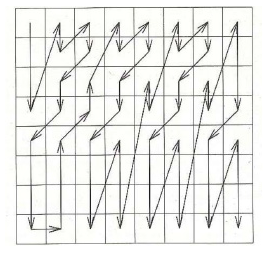
\includegraphics[width=10cm,height=10cm,keepaspectratio]{figuras/zigzag.png}
\end{center}
\caption{Método del zig-zag\cite{b1:2015}}
\label{fig_zigzag}
\end{figure}

El procesamiento de un GOP no es secuencial, al existir relaciones bidireccionales entre cierto tipo de frames. Al empezar un GOP, en primer lugar se procesa el I-frame. El siguiente frame a procesar será de tipo P, puesto que solamente necesita de este I-frame. Una vez procesados estos dos frames, los B-frames que están en medio serán decodificados. El proceso sigue alternando el procesamiento de P-frames con B-frames intermedios, hasta finalizar el GOP en cuestión, como se puede ver en \ref{fig_gop}.

\begin{figure}[ht!]
\begin{center}
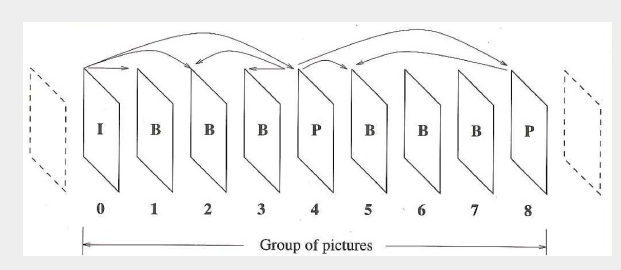
\includegraphics[width=10cm,height=10cm,keepaspectratio]{figuras/gop.png}
\end{center}
\caption{Procesamiento en GOP}
\label{fig_gop}
\end{figure}

\section{Procesamiento en sensores de imágenes} 
Existen principalmente dos tipos de sensores que se usan para capturar imágenes o vídeo: sensores CCD (del inglés \textit{Charge Coupled Device}) y sensores CMOS (del inglés \textit{Complementary Metal Oxide Semiconductor}). Ambos sensores se basan en el mismo principio que es capturar la máxima cantidad de luz que incide en el sensor y convertirla en una se\~al eléctrica que será transformada posteriormente en digital. Los sensores CMOS tratan los píxeles de forma individaul mientras que los sensores CCD se basan en la propagación de carga eléctrica mediante condensadores. En la actualidad, los sensores CMOS son ampliamente utilizados, sobre todo en dispositivos móviles, ya que los sensores CCD necesitan un chip adicional y son más costosos y grandes que los CMOS, por lo que en lo que sigue se detallará el funcionamiento de los sensores CMOS\cite{villalba:2015}. 

Un sensor CMOS consiste en una matrix de sensores de pixels, cada uno de ellos compuesto de un fotodetector y un amplificador activo. Cada uno de estos sensores de pixels captura información de un píxel en uno de los tres colores primarios (rojo, verde y azul) puesto que se aplica un filtro de color conocido como CFA (\textit{Color Filter Array}). Bayer es el CFA más utilizado, compuesto por un patrón de filtro que es la mitad verde, un cuarto azul y un cuarto rojo, debido a que el ojo humano es más sensible al color verde\ref{fig_cfa}\cite{b3:2012}. \\ 

\begin{figure}[ht!]
\begin{center}
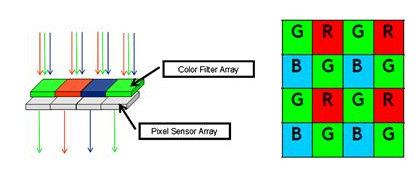
\includegraphics[width=10cm,height=10cm,keepaspectratio]{figuras/cfa.png}
\end{center}
\caption{Bayern CFA, \cite{b3:2012}}
\label{fig_cfa}
\end{figure}

Tras la aplicación del filtro CFA para cada píxel se tiene únicamente información sobre un color, lo que implica que se tiene que llevar a cabo un proceso para estimar los valores de los otros dos componentes del color. Esta estimación se puede realizar mediante distintas técnicas, todas ellas basadas en utilizar los valores de los píxels cercanos. Se pueden usar métodos sencillos como el del vecino más próximo (el píxel toma el valor del píxel que le precede) o el bilinear (toma como valor la media de sus vecinos en vertical y horizontal más próximos) u otros más complejos como pueden ser splines cúbicas, método de mínimos cuadrados o filtros direccionales\cite{b2:2005}.

Tras la conversión Bayer-RGB hay varias funciones que en función del dispositivo y sensor pueden aplicarse como pueden ser corrección del color o corrección gamma. \\

Hay que tener en cuenta que en este proceso el hardware tiene una influencia considerable. Cada sensor a pesar de pertenecer al mismo fabricante tiene peque\~nas imperfecciones o diferencias del resto que impactan directamente en la imagen obtenida. Esto es conocido como el ruido del sensor, que se aborda en la siguiente sección.

\section{Extracción del ruido en imágenes}
Los principales componentes del ruido en imágenes por imperfecciones del sensor son el FPN (\textit{Fixed Pattern Noise}) y el PRNU (\textit{Photo Response Non Uniformity}).

El ruido FPN se genera por la corriente oscura y depende también de la exposición y de la temperatura. Es un ruido independiente de las imperfecciones del sensor y es un ruido aditivo que es eliminado en algunas cámaras restando una capa de color negro.

El ruido PRNU es el mayoritario y es un ruido multiplicativo, lo que complica su eliminación. Está compuesto por dos ruidos: PNU (\textit{Pixel Non-Uniformity}) y por defectos de baja frecuencia como pueden ser la configuración del zoom, y la refracción de la luz en las lentes. Es el primero de estos dos componentes, el PNU, el que tiene que ver con la fabricación de los wafers de silicio y las imperfecciones en el proceso de fabricación, lo que hace que sea un atributo único de cada sensor. \\

La extracción del PRNU se basa en aplicar una función a la imagen original que elimine el ruido de la imagen, obteniendo la imagen limpia de ruido. Al substraer la imagen original de la imagen sin ruido obtenemos el ruido. En \cite{dabov:2007} usan el algoritmo BM3D y en \cite{gisolf:2013} proponen usar el algoritmo FSTV, en \cite{goljan:2006} usan transformadas de ondículas o \textit{wavelets} para eliminar el ruido. Este ruido puede estar contaminado por agentes externos, en consecuencia se han desarrollado técnicas como \textit{zero-mean}\cite{goljan:2008} o el filtro de Wiener\cite{wiki:wiener}.
